\section{Maior prefixo comum entre duas substrings}

\begin{frame}[fragile]{Maior prefixo comum entre duas substrings}

    \begin{itemize}
        \item O vetor de sufixos de $s$ pode ser utilizado para computar o maior prefixo 
            comum (\textit{longest common prefix -- LCP}) entre duas substrings de $s$

        \item A ideia central é calcular o maior prefixo comum entre os pares de sufixos
            adjacentes em $s_A(s)$

        \item Defina $lcp(i)$ como o tamanho do maior prefixo comum entre os sufixos
           $s_A[i]$ e $s_A[i + 1]$, com $i = 1, 2, \ldots, N - 1$
 
        \item Assim, o maior prefixo comum $LPC(i, j)$ entre os sufixos
            $s_A[i]$ e $s_A[j]$ é dado por
        \[
            LPC(i, j) = \min\ \lbrace\ lpc(i + 1), lpc(i + 2), \ldots, lpc(j)\ \rbrace
        \]

        \item Desde modo, o problema $LPC(i, j)$ é reduzido a um problema de \textit{range 
            minimun query -- RMQ}, o qual pode ser resolvido por meio de
            uma árvores de segmentos, por exemplo
    \end{itemize}

\end{frame}

\begin{frame}[fragile]{Algoritmo de Kasai}

    \begin{itemize}
        \item Uma vez computado o vetor de sufixos $s_A(s)$ de uma string $s$ de tamanho $N$,
            o algoritmo de Kasai permite computar os valores $lpc(i)$ em $O(N)$

        \item Considere dois sufixos consecutivos no vetor de sufixos, que iniciem nas posições
            $i$ e $j$ da string $s$, cujo maior prefixo comum entre eles tenha tamanho $k > 0$

        \item Se removidos os primeiros caracteres de cada um destes
            sufixos, serão obtidos os sufixos $i + 1$ e $j + 1$, os quais não são, 
            necessariamente, consecutivos no vetor de sufixos

        \item Contudo, estes novos sufixos tem, no mínimo, $k - 1$ caracteres comuns entre 
            seus prefixos

        \item Assim, $k - 1$ dentre as comparações feitas podem ser reaproveitadas para computar
            o próximo valor de $lcp$

        \item Um caso especial a ser considerado é o prefixo que ocupa a última posição
            do vetor de sufixos, que não terá um prefixo que o sucede
    \end{itemize}

\end{frame}

\begin{frame}[fragile]{Algoritmo de Kasai}

    \begin{itemize}
        \item Para determinar em qual posição inicia o $t$-ésimo sufixo do vetor de sufixos,
            é utilizado um vetor auxiliar $rank[t]$, que indica tal posição

        \item A variável $k$ que registrará o tamanho do maior prefixo comum deve iniciar com
            o valor zero

        \item No caso especial onde $rank[t] = N$, este valor $k$ deve ser reiniciado para
            o valor zero

        \item Nos demais casos, para cada valor de $i = 1, 2, \ldots, N$, o índice $j$ onde inicia
            o prefixo que o sucede $S[i..N]$ no vetor de sufixos será dado por 
                $j = s_A[rank[i] + 1]$

        \item O valor de $k$ deve ser incrementando enquanto $S[i + k]$ for igual a $S[j + k]$,
            respeitados os limites da string

        \item Assim, $lcp(rank[i]) = k$, e o valor $k$ deve ser decrementado para o próximo
            índice
    \end{itemize}

\end{frame}

\begin{frame}[fragile]{Visualização da construção do vetor $lcp$}

    \begin{figure}
        \centering

        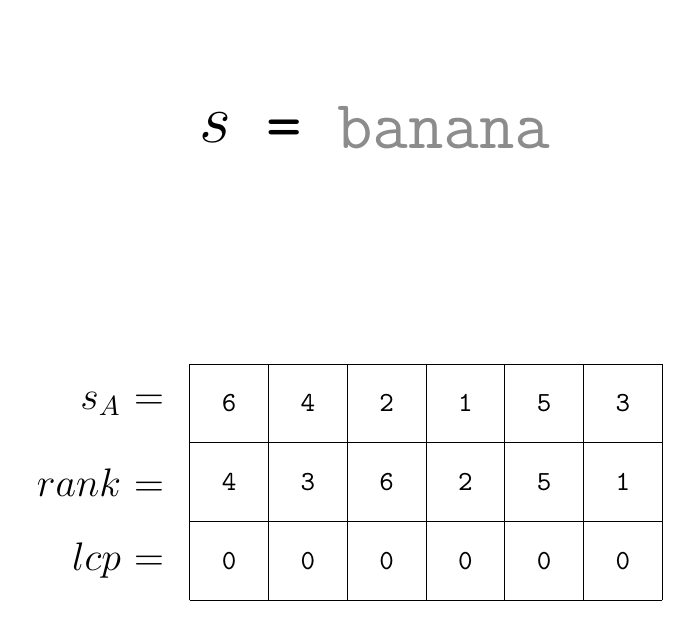
\begin{tikzpicture}
            \node[anchor=west] at (0, 5) { \Huge $s$ };
            \node[anchor=west] at (0.85, 5) { \Huge \texttt{= }\textcolor{gray!90}{\texttt{banana}} };
            \draw[opacity=0,<-] (2, 5.5) -- (2, 5.8) node[anchor=south] { $i$ };
            \draw[opacity=0,<-] (2.5, 4.5) -- (2.5, 4.2) node[anchor=north] { $j$ };

            \node[anchor=east] at (-0.2, 1.5) { \Large $s_A$ = };
            \draw (0, 1) grid (6, 2);
            \node[anchor=east] at (-0.2, 0.5) { \Large $rank$ = };
            \draw (0, 0) grid (6, 1);
            \node[anchor=east] at (-0.2, -0.5) { \Large $lcp$ = };
            \draw (0, -1) grid (6, 0);

            \node[opacity=0,anchor=west] at (-2.0, 3.0) { \Large $k = 0,$ };
            \node[opacity=0,anchor=west] at (1.0, 3.0) { \Large $i = 0,$ };
            \node[opacity=0,anchor=west] at (4.0, 3.0) { \Large $j = 0$ };

            \node at (0.5, 1.5) { \texttt{6} };
            \node at (1.5, 1.5) { \texttt{4} };
            \node at (2.5, 1.5) { \texttt{2} };
            \node at (3.5, 1.5) { \texttt{1} };
            \node at (4.5, 1.5) { \texttt{5} };
            \node at (5.5, 1.5) { \texttt{3} };

            \node at (0.5, 0.5) { {\texttt{4}} };
            \node at (1.5, 0.5) { {\texttt{3}} };
            \node at (2.5, 0.5) { {\texttt{6}} };
            \node at (3.5, 0.5) { {\texttt{2}} };
            \node at (4.5, 0.5) { {\texttt{5}} };
            \node at (5.5, 0.5) { {\texttt{1}} };

            \node at (0.5, -0.5) { {\texttt{0}} };
            \node at (1.5, -0.5) { {\texttt{0}} };
            \node at (2.5, -0.5) { {\texttt{0}} };
            \node at (3.5, -0.5) { {\texttt{0}} };
            \node at (4.5, -0.5) { {\texttt{0}} };
            \node at (5.5, -0.5) { {\texttt{0}} };


%            \node at (5.5, 0.5) { \textbf{\texttt{1}} };
        \end{tikzpicture}

    \end{figure}

\end{frame}

\begin{frame}[fragile]{Visualização da construção do vetor $lcp$}

    \begin{figure}
        \centering

        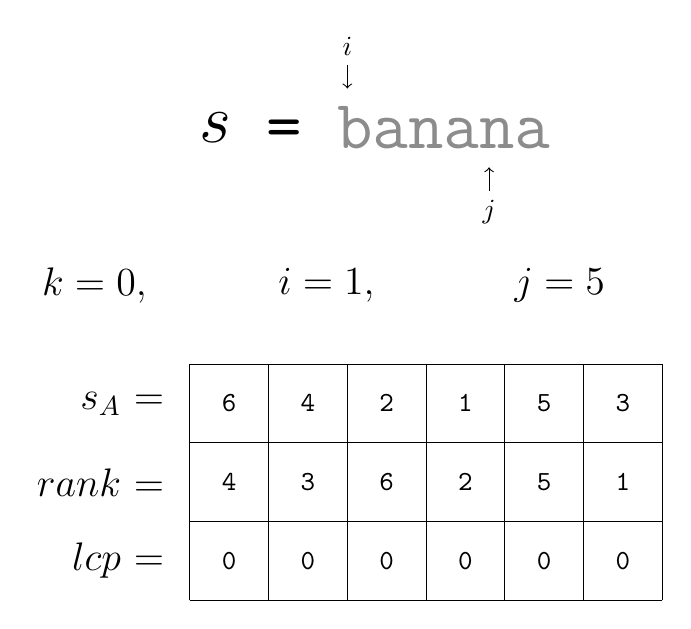
\begin{tikzpicture}
            \node[anchor=west] at (0, 5) { \Huge $s$ };
            \node[anchor=west] at (0.85, 5) { \Huge \texttt{= }\textcolor{gray!90}{\texttt{banana}} };
            \draw[opacity=1,<-] (2, 5.5) -- (2, 5.8) node[anchor=south] { $i$ };
            \draw[opacity=1,<-] (3.8, 4.5) -- (3.8, 4.2) node[anchor=north] { $j$ };

            \node[anchor=east] at (-0.2, 1.5) { \Large $s_A$ = };
            \draw (0, 1) grid (6, 2);
            \node[anchor=east] at (-0.2, 0.5) { \Large $rank$ = };
            \draw (0, 0) grid (6, 1);
            \node[anchor=east] at (-0.2, -0.5) { \Large $lcp$ = };
            \draw (0, -1) grid (6, 0);

            \node[opacity=1,anchor=west] at (-2.0, 3.0) { \Large $k = 0,$ };
            \node[opacity=1,anchor=west] at (1.0, 3.0) { \Large $i = 1,$ };
            \node[opacity=1,anchor=west] at (4.0, 3.0) { \Large $j = 5$ };

            \node at (0.5, 1.5) { \texttt{6} };
            \node at (1.5, 1.5) { \texttt{4} };
            \node at (2.5, 1.5) { \texttt{2} };
            \node at (3.5, 1.5) { \texttt{1} };
            \node at (4.5, 1.5) { \texttt{5} };
            \node at (5.5, 1.5) { \texttt{3} };

            \node at (0.5, 0.5) { {\texttt{4}} };
            \node at (1.5, 0.5) { {\texttt{3}} };
            \node at (2.5, 0.5) { {\texttt{6}} };
            \node at (3.5, 0.5) { {\texttt{2}} };
            \node at (4.5, 0.5) { {\texttt{5}} };
            \node at (5.5, 0.5) { {\texttt{1}} };

            \node at (0.5, -0.5) { {\texttt{0}} };
            \node at (1.5, -0.5) { {\texttt{0}} };
            \node at (2.5, -0.5) { {\texttt{0}} };
            \node at (3.5, -0.5) { \textbf{\texttt{0}} };
            \node at (4.5, -0.5) { {\texttt{0}} };
            \node at (5.5, -0.5) { {\texttt{0}} };


%            \node at (5.5, 0.5) { \textbf{\texttt{1}} };
        \end{tikzpicture}

    \end{figure}

\end{frame}

\begin{frame}[fragile]{Visualização da construção do vetor $lcp$}

    \begin{figure}
        \centering

        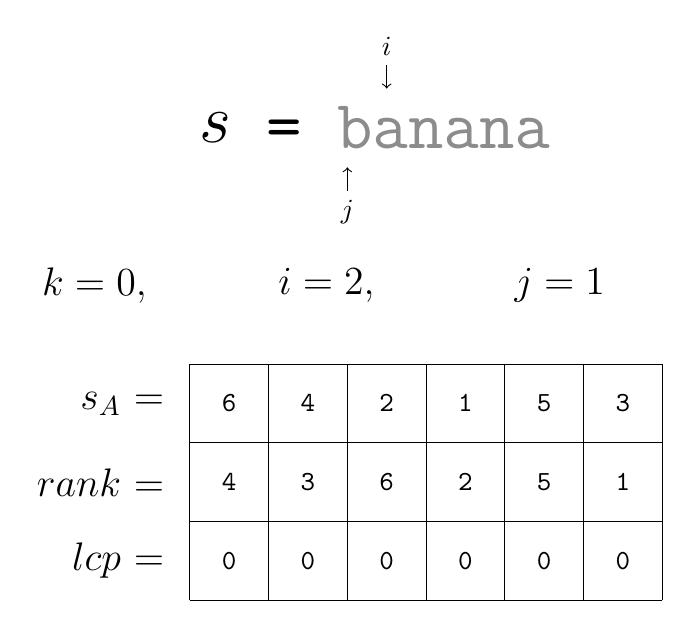
\begin{tikzpicture}
            \node[anchor=west] at (0, 5) { \Huge $s$ };
            \node[anchor=west] at (0.85, 5) { \Huge \texttt{= }\textcolor{gray!90}{\texttt{banana}} };
            \draw[opacity=1,<-] (2.5, 5.5) -- (2.5, 5.8) node[anchor=south] { $i$ };
            \draw[opacity=1,<-] (2.0, 4.5) -- (2.0, 4.2) node[anchor=north] { $j$ };

            \node[anchor=east] at (-0.2, 1.5) { \Large $s_A$ = };
            \draw (0, 1) grid (6, 2);
            \node[anchor=east] at (-0.2, 0.5) { \Large $rank$ = };
            \draw (0, 0) grid (6, 1);
            \node[anchor=east] at (-0.2, -0.5) { \Large $lcp$ = };
            \draw (0, -1) grid (6, 0);

            \node[opacity=1,anchor=west] at (-2.0, 3.0) { \Large $k = 0,$ };
            \node[opacity=1,anchor=west] at (1.0, 3.0) { \Large $i = 2,$ };
            \node[opacity=1,anchor=west] at (4.0, 3.0) { \Large $j = 1$ };

            \node at (0.5, 1.5) { \texttt{6} };
            \node at (1.5, 1.5) { \texttt{4} };
            \node at (2.5, 1.5) { \texttt{2} };
            \node at (3.5, 1.5) { \texttt{1} };
            \node at (4.5, 1.5) { \texttt{5} };
            \node at (5.5, 1.5) { \texttt{3} };

            \node at (0.5, 0.5) { {\texttt{4}} };
            \node at (1.5, 0.5) { {\texttt{3}} };
            \node at (2.5, 0.5) { {\texttt{6}} };
            \node at (3.5, 0.5) { {\texttt{2}} };
            \node at (4.5, 0.5) { {\texttt{5}} };
            \node at (5.5, 0.5) { {\texttt{1}} };

            \node at (0.5, -0.5) { {\texttt{0}} };
            \node at (1.5, -0.5) { {\texttt{0}} };
            \node at (2.5, -0.5) { \textbf{\texttt{0}} };
            \node at (3.5, -0.5) { {\texttt{0}} };
            \node at (4.5, -0.5) { {\texttt{0}} };
            \node at (5.5, -0.5) { {\texttt{0}} };


%            \node at (5.5, 0.5) { \textbf{\texttt{1}} };
        \end{tikzpicture}

    \end{figure}

\end{frame}

\begin{frame}[fragile]{Visualização da construção do vetor $lcp$}

    \begin{figure}
        \centering

        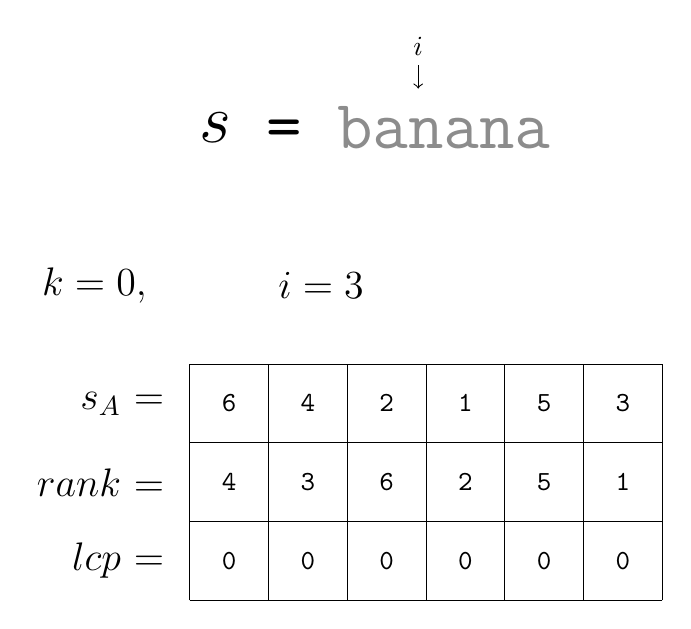
\begin{tikzpicture}
            \node[anchor=west] at (0, 5) { \Huge $s$ };
            \node[anchor=west] at (0.85, 5) { \Huge \texttt{= }\textcolor{gray!90}{\texttt{banana}} };
            \draw[opacity=1,<-] (2.9, 5.5) -- (2.9, 5.8) node[anchor=south] { $i$ };
            \draw[opacity=0,<-] (2.0, 4.5) -- (2.0, 4.2) node[anchor=north] { $j$ };

            \node[anchor=east] at (-0.2, 1.5) { \Large $s_A$ = };
            \draw (0, 1) grid (6, 2);
            \node[anchor=east] at (-0.2, 0.5) { \Large $rank$ = };
            \draw (0, 0) grid (6, 1);
            \node[anchor=east] at (-0.2, -0.5) { \Large $lcp$ = };
            \draw (0, -1) grid (6, 0);

            \node[opacity=1,anchor=west] at (-2.0, 3.0) { \Large $k = 0,$ };
            \node[opacity=1,anchor=west] at (1.0, 3.0) { \Large $i = 3$ };
            \node[opacity=0,anchor=west] at (4.0, 3.0) { \Large $j = 1$ };

            \node at (0.5, 1.5) { \texttt{6} };
            \node at (1.5, 1.5) { \texttt{4} };
            \node at (2.5, 1.5) { \texttt{2} };
            \node at (3.5, 1.5) { \texttt{1} };
            \node at (4.5, 1.5) { \texttt{5} };
            \node at (5.5, 1.5) { \texttt{3} };

            \node at (0.5, 0.5) { {\texttt{4}} };
            \node at (1.5, 0.5) { {\texttt{3}} };
            \node at (2.5, 0.5) { {\texttt{6}} };
            \node at (3.5, 0.5) { {\texttt{2}} };
            \node at (4.5, 0.5) { {\texttt{5}} };
            \node at (5.5, 0.5) { {\texttt{1}} };

            \node at (0.5, -0.5) { {\texttt{0}} };
            \node at (1.5, -0.5) { {\texttt{0}} };
            \node at (2.5, -0.5) { {\texttt{0}} };
            \node at (3.5, -0.5) { {\texttt{0}} };
            \node at (4.5, -0.5) { {\texttt{0}} };
            \node at (5.5, -0.5) { \textbf{\texttt{0}} };


%            \node at (5.5, 0.5) { \textbf{\texttt{1}} };
        \end{tikzpicture}

    \end{figure}

\end{frame}

\begin{frame}[fragile]{Visualização da construção do vetor $lcp$}

    \begin{figure}
        \centering

        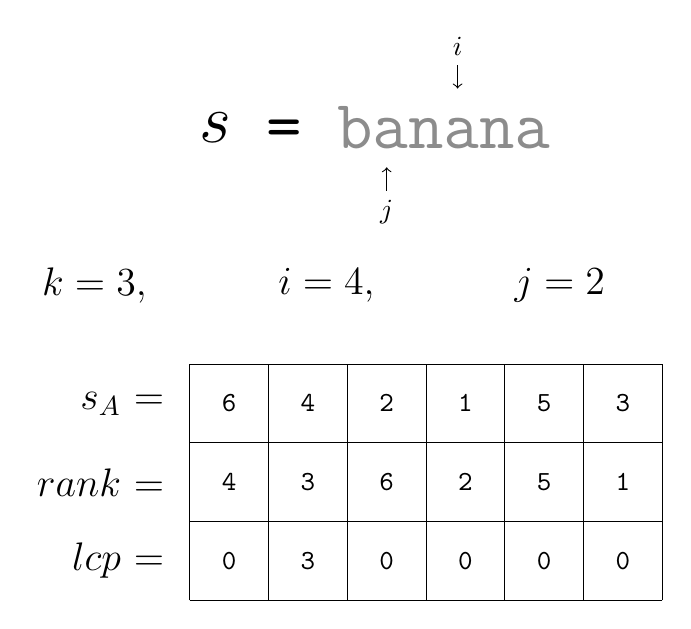
\begin{tikzpicture}
            \node[anchor=west] at (0, 5) { \Huge $s$ };
            \node[anchor=west] at (0.85, 5) { \Huge \texttt{= }\textcolor{gray!90}{\texttt{banana}} };
            \draw[opacity=1,<-] (3.4, 5.5) -- (3.4, 5.8) node[anchor=south] { $i$ };
            \draw[opacity=1,<-] (2.5, 4.5) -- (2.5, 4.2) node[anchor=north] { $j$ };

            \node[anchor=east] at (-0.2, 1.5) { \Large $s_A$ = };
            \draw (0, 1) grid (6, 2);
            \node[anchor=east] at (-0.2, 0.5) { \Large $rank$ = };
            \draw (0, 0) grid (6, 1);
            \node[anchor=east] at (-0.2, -0.5) { \Large $lcp$ = };
            \draw (0, -1) grid (6, 0);

            \node[opacity=1,anchor=west] at (-2.0, 3.0) { \Large $k = 3,$ };
            \node[opacity=1,anchor=west] at (1.0, 3.0) { \Large $i = 4,$ };
            \node[opacity=1,anchor=west] at (4.0, 3.0) { \Large $j = 2$ };

            \node at (0.5, 1.5) { \texttt{6} };
            \node at (1.5, 1.5) { \texttt{4} };
            \node at (2.5, 1.5) { \texttt{2} };
            \node at (3.5, 1.5) { \texttt{1} };
            \node at (4.5, 1.5) { \texttt{5} };
            \node at (5.5, 1.5) { \texttt{3} };

            \node at (0.5, 0.5) { {\texttt{4}} };
            \node at (1.5, 0.5) { {\texttt{3}} };
            \node at (2.5, 0.5) { {\texttt{6}} };
            \node at (3.5, 0.5) { {\texttt{2}} };
            \node at (4.5, 0.5) { {\texttt{5}} };
            \node at (5.5, 0.5) { {\texttt{1}} };

            \node at (0.5, -0.5) { {\texttt{0}} };
            \node at (1.5, -0.5) { \textbf{\texttt{3}} };
            \node at (2.5, -0.5) { {\texttt{0}} };
            \node at (3.5, -0.5) { {\texttt{0}} };
            \node at (4.5, -0.5) { {\texttt{0}} };
            \node at (5.5, -0.5) { {\texttt{0}} };


%            \node at (5.5, 0.5) { \textbf{\texttt{1}} };
        \end{tikzpicture}

    \end{figure}

\end{frame}

\begin{frame}[fragile]{Visualização da construção do vetor $lcp$}

    \begin{figure}
        \centering

        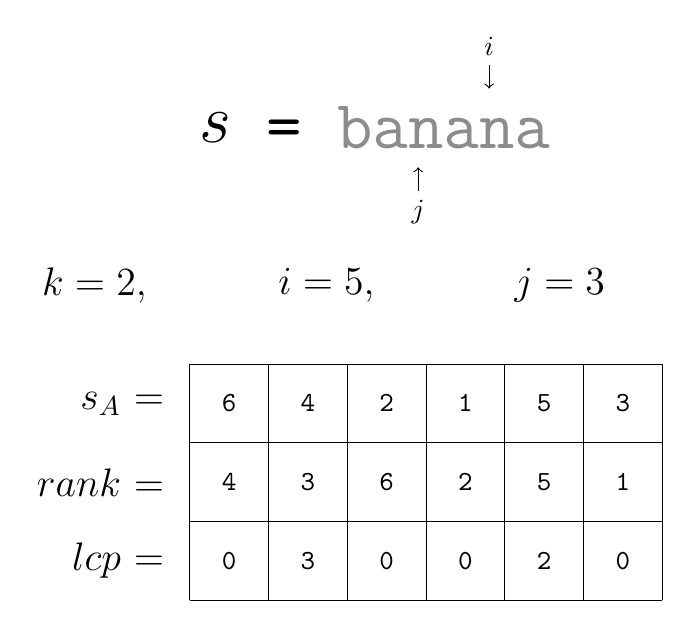
\begin{tikzpicture}
            \node[anchor=west] at (0, 5) { \Huge $s$ };
            \node[anchor=west] at (0.85, 5) { \Huge \texttt{= }\textcolor{gray!90}{\texttt{banana}} };
            \draw[opacity=1,<-] (3.8, 5.5) -- (3.8, 5.8) node[anchor=south] { $i$ };
            \draw[opacity=1,<-] (2.9, 4.5) -- (2.9, 4.2) node[anchor=north] { $j$ };

            \node[anchor=east] at (-0.2, 1.5) { \Large $s_A$ = };
            \draw (0, 1) grid (6, 2);
            \node[anchor=east] at (-0.2, 0.5) { \Large $rank$ = };
            \draw (0, 0) grid (6, 1);
            \node[anchor=east] at (-0.2, -0.5) { \Large $lcp$ = };
            \draw (0, -1) grid (6, 0);

            \node[opacity=1,anchor=west] at (-2.0, 3.0) { \Large $k = 2,$ };
            \node[opacity=1,anchor=west] at (1.0, 3.0) { \Large $i = 5,$ };
            \node[opacity=1,anchor=west] at (4.0, 3.0) { \Large $j = 3$ };

            \node at (0.5, 1.5) { \texttt{6} };
            \node at (1.5, 1.5) { \texttt{4} };
            \node at (2.5, 1.5) { \texttt{2} };
            \node at (3.5, 1.5) { \texttt{1} };
            \node at (4.5, 1.5) { \texttt{5} };
            \node at (5.5, 1.5) { \texttt{3} };

            \node at (0.5, 0.5) { {\texttt{4}} };
            \node at (1.5, 0.5) { {\texttt{3}} };
            \node at (2.5, 0.5) { {\texttt{6}} };
            \node at (3.5, 0.5) { {\texttt{2}} };
            \node at (4.5, 0.5) { {\texttt{5}} };
            \node at (5.5, 0.5) { {\texttt{1}} };

            \node at (0.5, -0.5) { {\texttt{0}} };
            \node at (1.5, -0.5) { {\texttt{3}} };
            \node at (2.5, -0.5) { {\texttt{0}} };
            \node at (3.5, -0.5) { {\texttt{0}} };
            \node at (4.5, -0.5) { \textbf{\texttt{2}} };
            \node at (5.5, -0.5) { {\texttt{0}} };


%            \node at (5.5, 0.5) { \textbf{\texttt{1}} };
        \end{tikzpicture}

    \end{figure}

\end{frame}

\begin{frame}[fragile]{Visualização da construção do vetor $lcp$}

    \begin{figure}
        \centering

        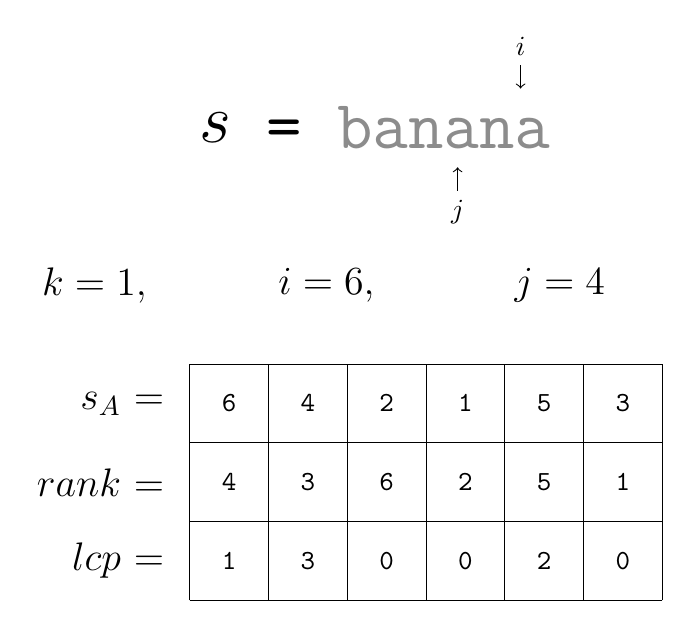
\begin{tikzpicture}
            \node[anchor=west] at (0, 5) { \Huge $s$ };
            \node[anchor=west] at (0.85, 5) { \Huge \texttt{= }\textcolor{gray!90}{\texttt{banana}} };
            \draw[opacity=1,<-] (4.2, 5.5) -- (4.2, 5.8) node[anchor=south] { $i$ };
            \draw[opacity=1,<-] (3.4, 4.5) -- (3.4, 4.2) node[anchor=north] { $j$ };

            \node[anchor=east] at (-0.2, 1.5) { \Large $s_A$ = };
            \draw (0, 1) grid (6, 2);
            \node[anchor=east] at (-0.2, 0.5) { \Large $rank$ = };
            \draw (0, 0) grid (6, 1);
            \node[anchor=east] at (-0.2, -0.5) { \Large $lcp$ = };
            \draw (0, -1) grid (6, 0);

            \node[opacity=1,anchor=west] at (-2.0, 3.0) { \Large $k = 1,$ };
            \node[opacity=1,anchor=west] at (1.0, 3.0) { \Large $i = 6,$ };
            \node[opacity=1,anchor=west] at (4.0, 3.0) { \Large $j = 4$ };

            \node at (0.5, 1.5) { \texttt{6} };
            \node at (1.5, 1.5) { \texttt{4} };
            \node at (2.5, 1.5) { \texttt{2} };
            \node at (3.5, 1.5) { \texttt{1} };
            \node at (4.5, 1.5) { \texttt{5} };
            \node at (5.5, 1.5) { \texttt{3} };

            \node at (0.5, 0.5) { {\texttt{4}} };
            \node at (1.5, 0.5) { {\texttt{3}} };
            \node at (2.5, 0.5) { {\texttt{6}} };
            \node at (3.5, 0.5) { {\texttt{2}} };
            \node at (4.5, 0.5) { {\texttt{5}} };
            \node at (5.5, 0.5) { {\texttt{1}} };

            \node at (0.5, -0.5) { \textbf{\texttt{1}} };
            \node at (1.5, -0.5) { {\texttt{3}} };
            \node at (2.5, -0.5) { {\texttt{0}} };
            \node at (3.5, -0.5) { {\texttt{0}} };
            \node at (4.5, -0.5) { {\texttt{2}} };
            \node at (5.5, -0.5) { {\texttt{0}} };


%            \node at (5.5, 0.5) { \textbf{\texttt{1}} };
        \end{tikzpicture}

    \end{figure}

\end{frame}


\begin{frame}[fragile]{Implementação da construção do vetor $lpc$}
    \inputsnippet{cpp}{84}{102}{codes/lcp.cpp}
\end{frame}

\begin{frame}[fragile]{Implementação da construção do vetor $lpc$}
    \inputsnippet{cpp}{104}{116}{codes/lcp.cpp}
\end{frame}

\begin{frame}[fragile]{Número de substrings distintas}

    \begin{itemize}
        \item Uma string $S$ de tamanho $N$ tem $N(N + 1)/2$ substrings no total

        \item Isto porque a substring $S[i..j]$ de $S$ pode ser caracterizada pelo par de índices
            $(i, j)$, com $1\leq i\leq j\leq N$

        \item O início de cada substring coincide com o ínicio de algum sufixo de $S$

        \item Deste modo, se $b = S[i..j] = S[r..s]$, isto significa que $b$ é prefixo comum entre              os sufixos $S[i..N]$ e $S[j..N]$

        \item Logo, todos os índices relacionados os maiores prefixos comuns entre dois
            prefixos consecutivos no vetor de prefixos geram substrings duplicadas

        \item Assim, se removidas as duplicatas do total de strings, resta o número de
            substrings distintas $D(S)$ de $S$

        \item Logo,
        \[
            D(S) = \frac{N(N + 1)}{2} - \sum_{i = 1}^{N - 1} lcp[i]
        \]
    \end{itemize}

\end{frame}

\begin{frame}[fragile]{Implementação da contagem de substrings distintas usando $lcp$}
    \inputsnippet{cpp}{118}{128}{codes/lcp.cpp}
\end{frame}
